\documentclass{article}
\usepackage{tikz}
\usepackage{pgfplots}
\usepackage{svg}
\usepackage{amsmath}
\usepackage{array}
\usepackage[skins]{tcolorbox}
\usepackage[version=4]{mhchem}
\usepackage[a4paper, total={6in, 9in}]{geometry}
\usepackage{fourier}
\usepackage{xymtex}
\usepackage{textcomp}
\usepackage{eurosym}
\usepackage{caption}
\usepackage{longtable}
\usepackage{float}
\usepackage{attachfile}
\usepackage{multirow}
\usepackage{amsfonts} 
\usepackage{tabularray}
\usepackage{colortbl}
\usepackage{xcolor}
\usepackage{graphicx}
\usepackage[table]{xcolor}
\UseTblrLibrary{booktabs}
\usepackage[bottom]{footmisc}

\captionsetup[table]{name=Tabella}
%<\pagenumbering{gobble}


\renewcommand*\contentsname{Indice}
\setcounter{tocdepth}{3}
%\setcounter{secnumdepth}{2}
\pgfplotsset{compat=1.15}


\title{Relazione di laboratorio - Periodo di un pendolo semplice}
\author{Federico Cesari}
\date{Aprile 2024}





%%%%%%%%%%%%%%%%%%%%%%%%%%%%%%%%%%%%%%%%%%%%%%%%%%%%%%%%%
%%				INIZIO DOC
%%%%%%%%%%%%%%%%%%%%%%%%%%%%%%%%%%%%%%%%%%%%%%%%%%%%%%%%%


\begin{document}
\begin{titlepage}
   \begin{center}
       \vspace*{1cm}
        
       \textbf{\LARGE Relazione di laboratorio - Esperienza di Poisson}
       
       \vspace{0.3cm}
       \large \textit{Rate di una sorgente radioattiva} \\
       
       \vspace{0.5cm}
       \Large Federico Cesari \\
       
       \small 1096759

			
		\vspace{1cm}
		\begin{center}
			\includegraphics[scale=1.2]{geiger.jpeg}	
		\end{center}
		
		

       \vfill
            
       
            
       \vspace{0.8cm}
     
       
            
       corso A\\
       Università degli studi di Torino, Torino\\
       3 marzo 2024\\
       
            
   \end{center}
\end{titlepage}

\tableofcontents

\newpage
\section{Scopo dell’esperienza}
L'esperienza di laboratorio ha lo scopo di studiare il periodo di un pendolo semplice del quale conosciamo le espressioni del periodo teorico (in condizioni ideali e prive di attrito) al variare della sua lunghezza e dell'angolo di partenza. Verrà quindi misurato il periodo e se ne osserverà la variazione in funzione dell'angolo, della lunghezza e della massa appesa ad esso.

\section{Premesse teoriche}
\textcolor{red}{aggiungi equazioni}

\section{Strumentazione}
\begin{table}[H]
	\centering
	\begin{tabular}{@{}ll@{}}
		\textbf{Strumento} & \textbf{Sensibilità} \\ \midrule
		Cr. Analogico      & $0.2$s               \\
		Cr. Digitale       & $0.01$s              \\
		Fotocellula        & $0.001$s             \\
		Goniometro         & $1^\circ$            \\
		Asta graduata      & $0.1$cm              \\
		Calibro            & $0.01$mm             \\
		Bilancia digitale  & $1$g                 \\ \bottomrule
	\end{tabular}
\end{table}





%%%%%%%%%%%%%%%%%%%%%%%%%%%%%%%%%%%%%%%%%%%%%%%%%%%%%%%%%
%%				SCELTA STRUMENTO
%%%%%%%%%%%%%%%%%%%%%%%%%%%%%%%%%%%%%%%%%%%%%%%%%%%%%%%%%




\section{Scelta strumento di misura}

Al fine di stabilire il migliore strumento di misura per le succesive misurazioni, registro 8 misure del periodo del pendolo prima con un angolo di partenza $\vartheta = 5^\circ$ e poi con $\vartheta = 30^\circ$ utilizzando un cronometro analogico, uno digitale e una fotocellula. Lo strumento che mostrerà discrepanze significative tra il periodo calcolato con $\vartheta = 5^\circ$ e $\vartheta = 30^\circ$ sarà quello utilizzato per i testi successivi. Procedo quindi con le misurazioni dei periodi del pendolo a cui è stata agganciata una sfera di massa $m = (110 \pm 1)g$

\textcolor{red}{sistema valori per C.Analogico e capire se aggiungere errori per T medi.}

\vspace{1cm}
\begin{minipage}{0.5\textwidth}
\begin{table}[H]
	\hspace{-1.3cm}
	\begin{tabular}{@{}lrrr@{}}
		&\textbf{C.Analogico} & \textbf{C. Digitale} & \textbf{Fotocellula} \\ \cmidrule(l){2-4} &\multicolumn{1}{l}{$T(s) \pm 0.2s$} & \multicolumn{1}{l}{$T(s) \pm 0.01s$}   & \multicolumn{1}{l}{$T(s) \pm 0.001s$}    \\ \cmidrule(l){2-4} 
		
		\multicolumn{1}{c}{}  
		& 1.6   & 1.63   & 1.702     \\
		\colorbox{orange!40}{$\vartheta = 5^\circ$}   & 1.7   & 1.65   & 1.703     \\
		& 1.5   & 1.60   & 1.703     \\ 
		& 1.7   & 1.71   & 1.703     \\
		& 1.7   & 1.71   & 1.703     \\
		& 1.7   & 1.65   & 1.702     \\
		& 1.6   & 1.70   & 1.703     \\
		& 1.7   & 1.70   & 1.703     \\ \arrayrulecolor{black!100}\specialrule{1.2pt}{0.5\jot}{0.5pc}
		
		$\mathbf{\bar{T}_{5}(s)}$ & \textbf{1.65}    & \textbf{1.67}  & \textbf{1.703}  \\
		$\sigma_{T_{5}}$   & 0.05    & 0.02  & 0.000 \\                          
	\end{tabular}
\end{table}
\end{minipage}
\begin{minipage}{0.5\textwidth}
\begin{table}[H]
	\centering
	\begin{tabular}{@{}lrrr@{}}
		&\textbf{C.Analogico} & \textbf{C. Digitale} & \textbf{Fotocellula} \\ \cmidrule(l){2-4} &\multicolumn{1}{l}{$T(s) \pm 0.2s$} & \multicolumn{1}{l}{$T(s) \pm 0.01s$}   & \multicolumn{1}{l}{$T(s) \pm 0.001s$}    \\ \cmidrule(l){2-4} 
		
		\multicolumn{1}{c}{}  
													& 1.8   & 1.65   & 1.733     \\
		\colorbox{blue!40}{$\vartheta = 30^\circ$}  & 1.7   & 1.67   & 1.733     \\
													& 1.6   & 1.70   & 1.733     \\ 
													& 1.7   & 1.62   & 1.733     \\
													
													& 1.7   & 1.70   & 1.731     \\
													& 1.8   & 1.72   & 1.733     \\
													& 1.7   & 1.80   & 1.733     \\
													& 1.6   & 1.69   & 1.732     \\ \arrayrulecolor{black!100}\specialrule{1.2pt}{0.5\jot}{0.5pc}

		$\mathbf{\bar{T}_{30}(s)}$ & \textbf{1.70}    & \textbf{1.69}  & \textbf{1.715}  \\
		$\sigma_ {T_{30}}$   & 0.08    & 0.03  & 0.0005 \\                          
	\end{tabular}
\end{table}
\end{minipage}
\vspace{1cm}

\noindent
Da questi primi set di dati noto subito che la deviazione standard dei periodi misurati dal cronometro digitale è più grande della sensibilità dello strumento, quindi dovrei scegliere la deviazione standard come errore sulla singola misura.


Invece per evidenziare quale dei tre strumenti fornisca periodi significativamente differenti per i due angoli di partenza sottopongo le coppie di periodi medi a un test Z:


\begin{table}[H]
	\centering
	\begin{tabular}{@{}lrr@{}}
		\toprule
		\multicolumn{1}{c}{Z} & \multicolumn{1}{l}{$\sigma_{\bar{T}_5}$} & \multicolumn{1}{l}{$\sigma_{\bar{T}_{30}}$} \\ \midrule
		$z_{\text{an.}}$      & \textit{\textbf{0.234}}                  & \textit{\textbf{0.234}}                   \\
		$z_{\text{dig.}}$     & \textit{\textbf{0.170}}                  & \textit{\textbf{0.132}}                   \\
		$z_{\text{fot.}}$     & \textit{\textbf{22.8}}                   & \textit{\textbf{14.2}}                    \\ \bottomrule
	\end{tabular}
\end{table}

Il test mostra che i periodi misurati con i cronometri analogico e digitale con ancgoli di partenza $\vartheta = 5^\circ$ e $\vartheta = 30^\circ$, risultano essere compatibili con livelli di significatività \textcolor{red}{maggiori dell'80\% (specifica bene i valori)}. Per quanto riguarda i periodi registrati con la fotocellula questi risultano \textcolor{red}{appartenere a popolazioni differenti} e posso quindi affermare che lo strumento che fornisce periodi significativamente differenti per i due angoli di partenza sia proprio la fotocellula.








%%%%%%%%%%%%%%%%%%%%%%%%%%%%%%%%%%%%%%%%%%%%%%%%%%%%%%%%%
%%				DIPENDENZA THETA   00000
%%%%%%%%%%%%%%%%%%%%%%%%%%%%%%%%%%%%%%%%%%%%%%%%%%%%%%%%%

\newpage
\section{Dipendenza dall’angolo}
La prima parte dell'esperienza consiste nel verificare la dipendenza di $T$, periodo del pendolo a cui è stata attaccata una sferetta di legno di massa $m = (10 \pm 1)g$, da $\vartheta$, angolo di oscillazione.  Per prima cosa si procede alla misurazoine della lunghezza del pendolo. Con l'asta graduata misuro prima la distanza da terra alla cima del pendolo ($L_C$) e poi la distanza da terra al centro della sfera appesa ($L_F$)\footnote{Avrei potuto misurare il diametro della sfera con il calibro e aggiungere il raggio della sfera successivamente invece che includerlo nelle misura di cima e fondo, tuttavia la sensibilità dell'asta e il fatto che questa non fosse perfettamente perpendicolare ha reso gli errori di $L_C$ e $L_F$ troppo grossolani rendendo così inutile la maggiore cura nella misura del raggio.}. 

\begin{table}[H]
	\centering
	\begin{tabular}{@{}p{3.6cm}p{3.6cm}@{}}
		\textbf{Cima} & \textbf{Fondo}\\ \midrule
		$L_C(\text{cm}) \pm 0.1\text{cm}$  & $L_F(\text{cm}) \pm 0.1\text{cm}$ \\ \midrule
		\multicolumn{1}{r}{89.0} \hspace{1.2cm} & \multicolumn{1}{r}{16.8}  \hspace{1.2cm}\\ \bottomrule
	\end{tabular}
\end{table}

Ricavo quindi la lunghezza del pendolo:

\[
l = L_C - L_F = (72.2 \pm 0.2) \text{cm}. \footnote{Propago l'errore linearmente ($\left(0.1 + 0.1 \right)\text{cm} = 0.2\text{cm}$) perché essendo solo due misure (per di più effettuate con un asta graduata imperfetta) rischio di sottostimare l'errore sommandolo in quadratura}
\] 

\subsection{Acquisizione dati}

A questo punto prendo tre misurazioni del periodo del pendolo per 6 angoli di partenza differenti. Con l'ausilio di un goniometro con sensibilità di $1^\circ$, partendo da un angolo di oscillazione di $5^\circ$, registro tre misure. Faccio lo stesso con  $\vartheta = 10^\circ$, $\vartheta = 15^\circ$  fino ad arrivare a un angolo di $30^\circ$. Finita la presa dati ottengo i seguenti periodi:


\vspace{0.7cm}
\begin{table}[H]
	\centering
	\begin{tabular}{@{}lrrrrrr@{}}
		& $\mathbf{5^\circ}$ & $\mathbf{10^\circ}$ & $\mathbf{15^\circ}$ & $\mathbf{20^\circ}$ & $\mathbf{25^\circ}$ & $\mathbf{30^\circ}$  \\ \cmidrule(l){2-7}   
		& $T(s) \pm 0.001s$ & $T(s) \pm 0.001s$   & $T(s) \pm 0.001s$ & $T(s) \pm 0.001s$ & $T(s) \pm 0.001s$ & $T(s) \pm 0.001s$  \\ \cmidrule(l){2-7} 
		
		\multicolumn{1}{c}{}  
		
		&1.703 & 1.706 & 1.710 & 1.715 & 1.723 & 1.730  \\
		&1.702 & 1.706 & 1.710 & 1.715 & 1.723 & 1.731 \\
		&1.701 & 1.706 & 1.710 & 1.715 & 1.723 & 1.731 \\
		
		\arrayrulecolor{black!100}\specialrule{1.2pt}{0.5\jot}{0.5pc}
		
		$\mathbf{\bar{T}(s)}$ & \textbf{1.702}    & \textbf{1.706}  & \textbf{1.710} & \textbf{1.715} & \textbf{1.723} &  \textbf{1.731}        
	\end{tabular}
\end{table}
\textcolor{red}{capire se aggiungere errori per T medi.}
\vspace{1cm}

\noindent
Dall'espressione del periodo del pendolo sappiamo che il periodo è direttamente proporzionale a $\sin\left(\vartheta/2\right)^2$, più precisamente:
\[
T = T_0 \left[ 1 + \frac{1}{4}\sin{\left(\vartheta/2\right)}^2 \right]
\]
Se dovessi riportare su un grafico i periodi sperimentali in funzione di $y = \sin{\left(\vartheta/2\right)}^2$ mi aspetto quindi un andamento lineare e più precisamente una retta del tipo

\[
T = T_0 + \frac{T_0}{4}y
\]

\noindent
Per verificare ciò mi avvalgo del metodo dei minimi quadrati...
\textcolor{red}{inserire qualche informazione a riguardo}

\newpage
\subsection{Retta di best-fit}
Appurato che $T$ e $\sin{\left(\vartheta/2\right)}^2$ siano \textit{teoricamente} linearmente correlati, è di mio interesse trovare quale retta della forma $T = a + by$ meglio interpola i dati sperimentali così da appurare se i valori misurati soddisfano la attesa teorica che $y$ sia lineare in $x$. 

Posso fare questo avvalendomi del metodo dei minimi quadrati che ha  proprio lo scopo di determinare i parametri che legano due variabili legate da essi, nel mio caso due variabili $x$ e $y$ legati da due parametri $A$ e $B$. Questo metodo necessita di alcune assunzioni importanti: 

\begin{enumerate}
	\item Le misure devono essere statisticamente indipendenti;
	\item Una delle due variabili (sceglierò la $x$) deve avere errori trascurabili rispetto all'altra \footnote{Giudico un errore come trascurabile rispetto all'altro quando si trovano in rapporto 1 a 3,4,5.}.
	\item Gli errori della variabile $y$ devono essere distribuiti normalmente.
\end{enumerate}
\textcolor{red}{preso letteralmente dal Cannelli}

\noindent
Per rispettare la seconda assunzione confronto gli errori relativi delle mie due variabili ($\delta_x$ è l'errore assoluto, $\delta_x/x$ è l'errore relativo).

\begin{minipage}{0.5\textwidth}
\begin{table}[H]
	\centering
	\begin{tabular}{@{}ccc@{}}
		\multicolumn{3}{c}{$\mathbf{T}$} \\ \midrule
		$T(s)$ & $\delta_T (s)$ & $\delta_T / T$ \\ \midrule
		1.702 & 0.001 & \textbf{0.000339} \\
		1.706 & 0.001 & \textbf{0.000338} \\
		1.710 & 0.001 & \textbf{0.000337} \\
		1.715 & 0.001 & \textbf{0.000336} \\
		1.723 & 0.001 & \textbf{0.000335} \\
		1.731 & 0.001 & \textbf{0.000333}  \\ \bottomrule   
	\end{tabular}
\end{table}
\end{minipage}
\begin{minipage}{0.5\textwidth}
\begin{table}[H]
	\centering
	\begin{tabular}{@{}ccc@{}}
		
		\multicolumn{3}{c}{$y = \mathbf{sin{\left(\vartheta/2\right)}^2}$} \\ \midrule
		$y$ & $\delta_y$ & $\delta_y / y$ \\ \midrule
		0.0019&0.00075 & \textbf{0.398} \\
		0.0076&0.0015 & \textbf{0.198}  \\
		0.017&0.0023 & \textbf{0.132}  \\ 
		0.030&0.0030 & \textbf{0.099}  \\
		0.047&0.0037 & \textbf{0.078}  \\
		0.067&0.0044 & \textbf{0.065}  \\ \bottomrule  
	\end{tabular}
\end{table}
\end{minipage}
\footnote{Lascio 3 cifre significative negli errori relativi del periodo per evidenziarne le piccole discrepanze.}
\vspace{1cm}

\noindent
Come si può leggere nelle tabelle l'errore associato alle misure dei periodi è perfettamente trascurabile rispetto a quello associato al seno, quindi scelgo di portare le misure del periodo sull'asse $x$ e quelle del seno sull'asse $y$. \\

\noindent
La funzione da linearizzare non è più 
\[
T = a + by
\]
ma bensì
\[
y = \mathbf{A} + \mathbf{B}T
\]



\begin{minipage}{0.3\textwidth}
\textcolor{red}{l'errore sulla x è da scrivere?}
\begin{table}[H]
	\centering
	\begin{tabular}{@{}ll@{}}
		$T(s) \pm \delta_T$ & $\sin{\left(\vartheta/2\right)}^2 \pm \delta_y$ \\ \midrule
		1.702&0.0019    \\
		1.706&0.0076    \\
		1.710&0.0170    \\
		1.715&0.0302    \\
		1.723&0.0468    \\
		1.731&0.0669    \\	\bottomrule
\end{tabular}
\end{table}
\end{minipage}
\begin{minipage}{0.7\textwidth}
\begin{figure}[H]
	\centering
	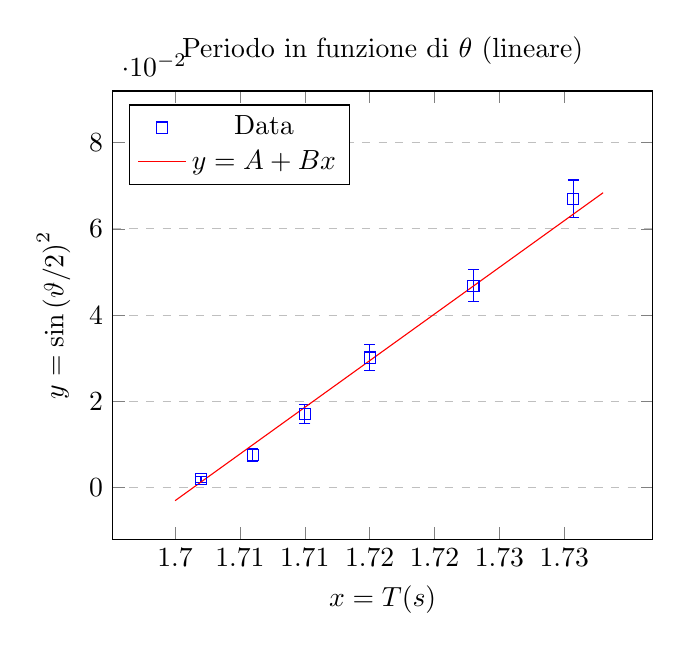
\begin{tikzpicture}
		\begin{axis}[
			title={Periodo in funzione di $\theta$ (lineare)},
			xlabel={$x = T(s)$},
			ylabel={$y = \sin{\left( \vartheta / 2\right) }^2$},
			xmin=1.7, xmax=1.732,
			ymin=0, ymax=0.08,
			xtick={1.7,1.705,1.71,1.715,1.72,1.725,1.73},
			ytick={0,0.02,0.04,0.06,0.08},
			legend pos=north west,
			ymajorgrids=true,
			grid style=dashed,
			enlargelimits=0.15,
			]
			
			\addplot[
			only marks,
			color=blue,
			mark=square,
			error bars/.cd,
			y dir=both, y explicit
			]
			coordinates {
				(1.702,0.0019027) +- (0,0.00075825)
				(1.706,0.0075961) +- (0,0.00151074)
				(1.710,0.0170371) +- (0,0.00225173)
				(1.715,0.0301537) +- (0,0.00297558)
				(1.723,0.0468461) +- (0,0.00367678)
				(1.7307,0.0669873) +- (0,0.00435)
			};
			\addplot[
				domain=1.7:1.733, 
				samples=100, 
				color=red, 
				] 
				{2.16490*x -3.68337};
			\node[] at (axis cs: 1.73,1) {absolute in pgfplots coordinates};
			\legend{Data,$y=A+Bx$}
		\end{axis}
	\end{tikzpicture}
\end{figure}
\end{minipage}
\[
\mathbf{A} = -3.68 \qquad \mathbf{\sigma_A} = 0.18
\]
\[
\mathbf{B} = 2.16 \qquad \mathbf{\sigma_B} = 0.10
\]

\vspace{1.5cm}
\noindent
La retta di "best-fit" può fornire altre importanti informazioni: per esempio nella retta 
\[
T = T_0 + \frac{T_0}{4}\sin{\left(\vartheta/2\right)}^2
\]
il termine noto della retta è $T_0$ che rappresenta il periodo delle piccole oscillazioni. Nel mio caso invece (ho il seno in funzione di $T$) la retta è espressa come
\[
\sin{\left(\vartheta/2\right)}^2 = 4\frac{T}{T_0} - 4
\]
nella quale $T_0$ compare a denominatore del coefficiente angolare della retta. Posso allora ricavarlo imponendo
\[
B =  4\frac{1}{T_0} \qquad T_0 = \frac{4}{B} 
\]
\textcolor{red}{a cosa mi dovrebbe servire trovare il periodo delle piccole oscillazioni?}

\noindent
Ho quindi trovato anche il valore sperimentale del periodo delle piccole oscillazioni del mio pendolo:
\[
\mathbf{T_0} = (1.85 \pm 0.09)\text{s}
\]
\footnote{L'errore di $T_0$ è $\sigma_{T_0} = \sqrt{\left(\frac{\partial T_0}{\partial B}\sigma_{B}\right)^2} = \left|\frac{\partial T_0}{\partial B}\sigma_{B}\right| = \frac{4}{B^2}\sigma_B$}

\subsubsection{Test del chi quadro}
Visti i risultati ottenuti assumo che la retta trovata di parametri $\mathbf{A}$ e $\mathbf{B}$ si adatti bene all'andamento dei miei dati. Per assicurarmene effettuo un test del $\chi^2$

\paragraph{Ipotesi nulla} La retta $y = A + Bx$ descrive bene l'andamento dei dati osservati sperimentalmente.

\vspace{0.7cm}
\begin{table}[H]
	\centering
	\begin{tabular}{lr} 
		Livello di significatività $\alpha$		&$\quad 0.05$  \\
		Valore di $\chi ^2$             	& $\quad 4.29$       \\
		Numero di gradi di libertà      	& $\quad (6-2) = 4$         \\   
		Valore di $\chi ^2$ critico     	& $\quad 9.49$
	\end{tabular}
\end{table}
\vspace{0.7cm}

\paragraph{Conclusione test} Il valore del $\chi^2$ ottenuto risulta essere minore del valore critico, posso quindi accettare l'ipotesi nulla e affermare che nei livelli di significatività scelti la retta $y = A + Bx$ descrive in modo accettabile l'andamento dei miei dati.

\subsubsection{Test Z}
Infine, appurato che la retta $y = A + Bx$ è una buona rappresentazione dell'andamento dei miei dati, mi interessa capire se l'andamento teorico lo è. Voglio quindi capire se l'equazione 
\[
\sin{\left(\vartheta/2\right)}^2 = 4\frac{T}{T_0} - 4
\]

che ha come parametri teorici
\[
A_\text{teo} = -4 \qquad B_\text{teo} =  \frac{4}{T_0}
\]
si adatta bene ai miei dati. Scelgo quindi un livello di significa $\alpha = 0.05$ con $z_{\text{critico}} = 1.96$ ed eseguo il test.

\paragraph{Ipotesi nulla} I valori $A_{\text{teo}}$, $\mathbf{A}$ e  $B_{\text{teo}}$, $\mathbf{B}$ sono a due a due compatibili.

\vspace{0.7cm}
\begin{minipage}{0.5\textwidth}
\begin{table}[H]
	\centering
	\begin{tabular}{lr} 
		Livello di significatività $\alpha$		&$\quad 0.05$  \\
		\textbf{B} sperimentale				& $\quad2.16 \pm  0.10$\\
		\textbf{B} teorico					& $\quad4/T_0$ \\
		$z_{B}$ osservato 					& $\quad$1.78 \\
		Valore di $Z$ critico     	& $\quad 1.96$
	\end{tabular}
\end{table}
\end{minipage}
\begin{minipage}{0.5\textwidth}
\begin{table}[H]
	\centering
	\begin{tabular}{lr} 
		Livello di significatività $\alpha$		&$\quad 0.05$  \\
		\textbf{A} sperimentale             	& $\quad-3.68 \pm 0.18 $     \\
		\textbf{A} teorico					&  $\quad-4$\\
		$z_{A}$ osservato					& 1.79 \\ 
		Valore di $Z$ critico     	& $\quad 1.96$
	\end{tabular}
\end{table}
\end{minipage}
\vspace{0.7cm}

\paragraph{Conclusione test} Poiché sia per $\mathbf{A}$ sia per $\mathbf{B}$ risulta che $z_{\text{oss}}$ < $z_{\text{critico}}$ posso affermare che entrambi sono compatibili con i rispettivi valori teorici nei livelli di significaticità scelti e che quindi l'equazione teorica della retta è una buona rappresentazione dell'andamento dei miei dati.

\subsection{Determinazione dell'accelerazione di gravità g}
Sappiamo le piccole oscillazioni del pendolo hanno periodo descritto da
\[
T_0 = 2\pi \sqrt{\frac{l}{g}} 
\]
dove $l$ è la distanza dalla cima del pendolo al centro di massa della sfera appesa ad esso, nel mio caso $l = (72.2 \pm 0.2)$cm. Dall'equazione precedente (e ricordando che $T_0 = 4/B$) troviamo l'espressione dell'accelerazione di gravità:
\[
g = \frac{\pi^2b^2l}{4}
\]

con errore associato

\[
\sigma_g = \sqrt{\left(\frac{\partial g}{\partial l} \right)^2\sigma_l^2 + \left(\frac{\partial g}{\partial B} \right)^2 \sigma_B^2}  \quad = \quad 	\sqrt{\left(\frac{B^2\pi^2}{4}\right)^2 \sigma_l^2 + \left( \frac{lB\pi^2}{2}  \right)^2 \sigma_B^2}	 
\]


\noindent
Posso quindi conlcudere e scrivere il valore sperimentale di $\mathbf{g}$ determinato dalle mie misurazioni:
\[
\mathbf{g} = (830 \pm 81)\text{cm}\cdot \text{s}^{-2}
\]
\noindent
Sapendo che il valore dell'accelerazione di gravità terrestre vale circa $9.81ms^{-2}$ si nota subito la differenza con il $g$ determinato sperimentalmente che risulta essere sottostimato del $15\%$. Tale sottostima è da imputare alla misura della lunghezza del pendolo $l$ e al valore di $B$. (\textcolor{red}{inserire il fatto che B sia il rapporto sin / T?}) Per capire chi influenza maggiormente la bontà del risultato ottenuto calcolo l'errore associato a $g$ "più grossolanamente" così da evidenziare in modo più facile il "colpevole":

\[
		\frac{\sigma_g}{g} = \frac{\sigma_l}{l} + 2\frac{\sigma_b}{b} 
\]
\[
		\approx \quad 0.28 \% + 9.72 \% \quad \approx  \quad 10\%	
\]

trovando quindi che l'errore su $B$ è quello che più influisce sull'accuratezza del valore di $g$ calcolato.
\\

\subsubsection{Test Z}
Infine è bene verificare l'accordo tra $g$ da me calcolato e $G = 9.81 ms^{-2}$. In linea teorica infatti mi aspetto che i due siano uguali e che eventuali discrepanze siano dovute unicamente al caso. Applico allora un Test Z:

\paragraph{Ipotesi nulla} Il valore $g$ da me calcolato è compatibile con il valore vero $G$ accelerazione di gravità terrestre.

\vspace{0.7cm}
\begin{table}[H]
	\centering
	\begin{tabular}{lr}
		Livello di significatività $\alpha$	& $\quad 0.05$  \\
		Valore di $z_\text{oss}$             	& $\quad 1.86$  \\
		Valore di $z_{\text{critico}}$ 		& $\quad 1.96$  \\ 
	\end{tabular}
\end{table}
\vspace{0.7cm}

\noindent
Poiché $z_\text{oss}$ < $z_{\text{critico}}$ posso concludere che con un livello di significatività del 5\% $g$ risulta essere compatibile con $G$.


\newpage
\subsection{Parabola di best-fit}
Poiché nel processo di determinazione della retta di best-fit è risultato opportuno studiare la funzione $T(y)$ con $y = \sin{\left( \vartheta / 2\right)}^2$ per poter studiare la funzione in forma parabolica basta prendere $y =  \sin{\left( \vartheta / 2\right)}$.

Come ho fatto per il fit lineare, controllo quale delle due variabili, $T$ e $ \sin{\left( \vartheta / 2\right)}$, ha errore relativo trascurabile rispetto a quello dell'altra.


\begin{minipage}{0.5\textwidth}
	\begin{table}[H]
		\centering
		\begin{tabular}{@{}ccc@{}}
			\multicolumn{3}{c}{$\mathbf{T}$} \\ \midrule
			$T(s)$ & $\delta_T (s)$ & $\delta_T / T$ \\ \midrule
			1.702 & 0.001 & \textbf{0.000339} \\
			1.706 & 0.001 & \textbf{0.000338} \\
			1.710 & 0.001 & \textbf{0.000337} \\
			1.715 & 0.001 & \textbf{0.000336} \\
			1.723 & 0.001 & \textbf{0.000335} \\
			1.731 & 0.001 & \textbf{0.000333}  \\ \bottomrule   
		\end{tabular}
	\end{table}
\end{minipage}
\begin{minipage}{0.5\textwidth}
	\begin{table}[H]
		\centering
		\begin{tabular}{@{}ccc@{}}
			
			\multicolumn{3}{c}{$y = \mathbf{sin{\left(\vartheta/2\right)}}$} \\ \midrule
			$y$ & $\delta_y$ & $\delta_y / y$ \\ \midrule
			0.044 & 0.00869 & \textbf{0.199} \\
			0.087 & 0.00867 & \textbf{0.099} \\
			0.131 & 0.00863 & \textbf{0.066} \\
			0.174 & 0.00857 & \textbf{0.049} \\
			0.216 & 0.00849 & \textbf{0.039} \\
			0.259 & 0.00840 & \textbf{0.032}  \\ \bottomrule  
		\end{tabular}
	\end{table}
\end{minipage}
\vspace{1cm}


\noindent
Se per il fit lineare ho potuto invertire le variabili con l'intento di mettere sull'asse $x$ la variabile con errore trascurabile, per il fit parabolico non posso farlo; andrei infatti a graficare l'equazione di una radice quadrata perdendo di fatto le informazioni che mi interessa trovare: i parametri \textbf{A}, \textbf{B} e \textbf{C} della parabola che meglio interpola i dati sperimentali.

\vspace{1cm}
\hspace{-1cm}
\begin{minipage}{0.7\textwidth}
\begin{figure}[H]
	\centering
	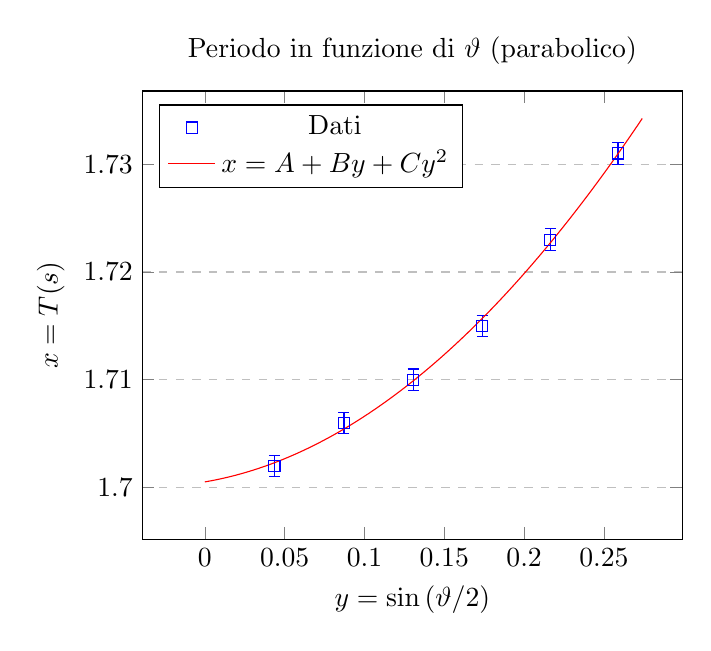
\begin{tikzpicture}
		\begin{axis}[
			title={Periodo in funzione di $\vartheta$ (parabolico)},
			ylabel={$x = T(s)$},
			xlabel={$y = \sin{\left( \vartheta / 2\right) }$},
			xmin=0, xmax=0.26,
			ymin=1.700, ymax=1.732,
			xtick={},
			ytick={},
			tick label style={/pgf/number format/fixed},
			legend pos=north west,
			ymajorgrids=true,
			grid style=dashed,
			enlargelimits=0.15,
			]
			
			\addplot[
			only marks,
			mark=square,
			color=blue,
			error bars/.cd,
			y dir=both, y explicit
			]
			coordinates {
				(0.0436194,1.702) +- (0,0.001)
				(0.0871557,1.706) +- (0,0.001)
				(0.1305262,1.710) +- (0,0.001)
				(0.1736482,1.715) +- (0,0.001)
				(0.2164396,1.723) +- (0,0.001)
				(0.2588190,1.731) +- (0,0.001)
			};
			\addplot[
			domain=0:0.274, 
			samples=100, 
			color=red, 
			] 
			{0.35725602*x^2 + 0.0252062*x + 1.700522};
			\legend{Dati,$x=A+By+Cy^2$}
		\end{axis}
	\end{tikzpicture}
\end{figure}
\end{minipage}
\begin{minipage}{0.3\textwidth}
\begin{table}[H]
	\centering
	\begin{tabular}{@{}rr@{}}
		$T(s) \pm \delta_T$ & $\sin{\left(\vartheta/2\right)} \pm \delta_y$ \\ \midrule
		1.702&0.044    \\
		1.706&0.087    \\
		1.710&0.130    \\
		1.715&0.174    \\
		1.723&0.216    \\
		1.731&0.259    \\	\bottomrule
	\end{tabular}
\end{table}	
\end{minipage}
\vspace{0.8cm}
\[
\mathbf{A} = 1.70 \qquad \mathbf{\sigma_A} = 0.0018
\]
\[
\mathbf{B} = 0.0252 \qquad \mathbf{\sigma_B} = 0.0273
\]
\[
\mathbf{C} = 0.357 \qquad \mathbf{\sigma_C} = 0.088
\]
\vspace{0.2cm}


\subsubsection{Test del chi quadro}
Assumendo che la parabola trovata $x=A+By+Cy^2$ si adatti bene all'andamento dei dati scelgo un livello di significatività $\alpha = 0.05$ ed eseguo il test.

\paragraph{Ipotesi nulla} La parabola con parametri \textbf{A},\textbf{B} e \textbf{C} si adatta bene all'andamento dei miei dati.

\vspace{0.7cm}
\begin{table}[H]
	\centering
	\begin{tabular}{lr} 
		Livello di significatività $\alpha$		&$\quad 0.05$  \\
		Valore di $\chi ^2$             		& $\quad 0.96$       \\
		Numero di gradi di libertà      		& $\quad (6-3) = 3$         \\   
		Valore di $\chi ^2$ sospetto			& $\quad 0.35$ \\
		Valore di $\chi ^2$ critico     		& $\quad 7.8$
	\end{tabular}
\end{table}
\vspace{0.7cm}

\paragraph{Conclusione test}
Il valore del chi quadro calcolato risulta essere compreso tra il valore sospetto e quello critico: $\chi^2_\text{sospetto} < \chi ^2 < \chi^2_\text{critico}$ posso quindi affermare che, con livello di significatività del 5\%, la parabola descritta dai parametri \textbf{A},\textbf{B} e \textbf{C} si adatta bene all'andamento dei miei dati.


\subsubsection{Test Z}
Per constatare se la parabola descrive bene l'andamento dei miei dati (graficamente sembrerebbe farlo) vado a confrontare i parametri ottenuti con quelli teorici. La parabola teorica 
\[
T = T_0 + \frac{T_0}{4}\sin{(\vartheta/2)}^2
\]
ha come parametri teorici
\[
A_\text{teo} = T_0 \qquad B_\text{teo} = 0 \qquad C_\text{teo} =  \frac{T_0}{4} 
\]

\noindent
Procedo quindi con un Test Z per verificare la compatibilità tra i valori:

\paragraph{Ipotesi nulla} I parametri della parabola sperimentale sono compatibili con i parametri della parabola teorica.

\vspace{0.7cm}
\begin{minipage}{0.5\textwidth}
	\begin{table}[H]
		\centering
		\begin{tabular}{lr} 
			Livello di significatività $\alpha$		&$\quad 0.05$  \\
			\textbf{A} sperimentale				& $\quad1.700 \pm 0.0018 $\\
			\textbf{A} teorico					&  $\quad1.704$ \\
			$z_{A}$ osservato 					& $\quad$1.78 \\
			Valore di $Z$ critico     	& $\quad 1.96$
		\end{tabular}
	\end{table}
\end{minipage}
\begin{minipage}{0.5\textwidth}
	\begin{table}[H]
		\centering
		\begin{tabular}{lr} 
			Livello di significatività $\alpha$		&$\quad 0.05$  \\
			\textbf{B} sperimentale				& $\quad0.0252 \pm  0.0273$	\\
			\textbf{B} teorico					& $\quad 0$ \\
			$z_{B}$ osservato 					& $\quad$1.78 \\
			Valore di $Z$ critico     	& $\quad 1.96$
		\end{tabular}
	\end{table}
\end{minipage}

\begin{table}[H]
		\centering
		\begin{tabular}{lr} 
			Livello di significatività $\alpha$		&$\quad 0.05$  \\
			\textbf{C} sperimentale             	& $\quad0.357 \pm 0.088$     \\
			\textbf{C} teorico					&  $\quad 0.426 $\\
			$z_{C}$ osservato					& 1.79 \\ 
			Valore di $Z$ critico     	& $\quad 1.96$
		\end{tabular}
\end{table}
\vspace{0.7cm}

\paragraph{Conclusione test}
Poiché ogni $z_\text{oss}$ risulta minore dello $z_\text{critico}$,  concludo che con un livello di significatività del 5\%, tutti i parametri risultano essere compatibili con le aspettative teoriche.

%%%%%%%%%%%%%%%%%%%%%%%%%%%%%%%%%%%%%%%%%%%%%%%%%%%%%%%%%
%%				DIPENDENZA ELLE     LLLLL
%%%%%%%%%%%%%%%%%%%%%%%%%%%%%%%%%%%%%%%%%%%%%%%%%%%%%%%%%

\newpage
\section{Dipendenza dalla lunghezza}
\subsection{Acquisizione dati}
Per prima cosa procedo con le misurazioni di 5 pendoli di 5 diverse lunghezze. Con l'ausilio dell'asta graduata, come fatto in precedenza, misuro prima la distanza da terra alla cima del pendolo ($L_C$) e poi la distanza da terra al centro della sfera appesa ($L_F$). Come errore su $l$ associo 2 volte la sensibilità dell'asta.
\[
l_i = L_C - L_{F_i} \qquad i= 1, \dots, 5
\]

\begin{table}[H]
	\centering
	\begin{tabular}{@{}ccccc@{}}
		$\mathbf{l_1}$ & $\mathbf{l_2}$ & $\mathbf{l_3}$ & $\mathbf{l_4}$ & $\mathbf{l_5}$  \\ \midrule
		$l_1(\text{cm}) \pm 0.2\text{cm}$  & $l_2(\text{cm}) \pm 0.2\text{cm}$  & $l_3(\text{cm}) \pm 0.2\text{cm}$ & $l_4(\text{cm}) \pm 0.2\text{cm}$ & $l_5(\text{cm}) \pm 0.2\text{cm}$\\ \midrule
		\multicolumn{1}{r}{60.2} & \multicolumn{1}{r}{26.7} & \multicolumn{1}{r}{14.5} & \multicolumn{1}{r}{63.0} & \multicolumn{1}{r}{54.8}\\ \bottomrule
	\end{tabular}
\end{table}



Come per lo studio del periodo in funzione dell'angolo di oscillazione, anche in questo caso registro tre misure del periodo per ogni sua lunghezza lunghezza scelta per un totale di 5 lunghezze differenti.

\vspace{0.7cm}
\begin{table}[H]
	\centering
	\begin{tabular}{@{}lrrrrr@{}}
		& $\mathbf{l_1}$ & $\mathbf{l_2}$ & $\mathbf{l_3}$ & $\mathbf{l_4}$ & $\mathbf{l_5}$  \\ \cmidrule(l){2-6}   
		& $T(s) \pm 0.001s$ & $T(s) \pm 0.001s$   & $T(s) \pm 0.001s$ & $T(s) \pm 0.001s$ & $T(s) \pm 0.001s$  \\ \cmidrule(l){2-6} 
		
		\multicolumn{1}{c}{}  
		
		& 1.504 & 0.964 & 0.663 & 1.556 & 1.437 \\
		& 1.504 & 0.962 & 0.662 & 1.558 & 1.437 \\
		& 1.502 & 0.962 & 0.663 & 1.555 & 1.436 \\
		
		\arrayrulecolor{black!100}\specialrule{1.2pt}{0.5\jot}{0.5pc}
		
		$\mathbf{\bar{T}(s)}$ & \textbf{1.503} & \textbf{0.9627} & \textbf{0.6627} & \textbf{1.556} & \textbf{1.437}     
	\end{tabular}
\end{table}
\textcolor{red}{capire se aggiungere errori per T medi.}


	

\vspace{1cm}


\subsection{Retta di best-fit}
Ricordando l'espressione teorica del periodo del pendolo è possibile evidenziare la relazione lineare tra $T^2$ (il periodo al quadrato) e  $l$ (lunghezza del pendolo):
\[
T = 2\pi \sqrt{\frac{l}{g}} \left( 1 + \frac{1}{4}\sin{\left(\vartheta/2\right)}^2 \right) \qquad T^2 = 4 \pi^2 \frac{l}{g} \left( 1 + \frac{1}{4}\sin{\left(\vartheta/2\right)}^2 \right)^2
\]
\[
T^2 = C_3 l
\]
con $C_3 =  \frac{4 \pi^2}{g} \left( 1 + \frac{1}{4}\sin{\left(\vartheta/2\right)}^2 \right)^2$ \\

\noindent
Per applicare al meglio il metodo dei minimi quadrati controllo sempre quale delle due variabili ha errore relativo più piccolo.

\begin{minipage}{0.5\textwidth}
	\begin{table}[H]
		\centering
		\begin{tabular}{@{}ccc@{}}
			\multicolumn{3}{c}{$\mathbf{T^2}$} \\ \midrule
			$T^2(s)$ & $\delta_{T^2} (s)$ & $\delta_{T^2} / T^2$ \\ \midrule
			2.26 & 0.00301 & \textbf{0.00133 }\\
			0.926 & 0.00193 & \textbf{0.00208} \\
			0.439 & 0.00133 & \textbf{0.00302} \\
			2.422 & 0.00311 & \textbf{0.00129} \\
			2.064 & 0.00287 & \textbf{0.00139}  \\ \bottomrule   
		\end{tabular}
	\end{table}
\end{minipage}
\begin{minipage}{0.5\textwidth}
	\begin{table}[H]
		\centering
		\begin{tabular}{@{}ccc@{}}
			\multicolumn{3}{c}{\textbf{l}} \\ \midrule
			$l$ & $\delta_l$ & $\delta_l / l$ \\ \midrule
			60.20 & 0.2 & \textbf{0.00332} \\
			26.70 & 0.2 & \textbf{0.00749} \\
			14.50 & 0.2 & \textbf{0.0138} \\
			63.00 & 0.2 & \textbf{0.00317} \\
			54.80 & 0.2 & \textbf{0.00364} \\ \bottomrule  
		\end{tabular}
	\end{table}
\end{minipage}
\vspace{1cm}

\noindent
L'errore associato a $l$ risulta essere significativamente più grande di quello su $T^2$ quindi decido di invertire la relazione per poter mettere sull'asse $x$ il periodo al quadrato:
\[
 l = \frac{1}{C_3} T^2
\]

\[
\mathbf{A} = 3.745 \qquad \mathbf{\sigma_A} = 0.204
\]
\[
\mathbf{B} = 24.713 \qquad \mathbf{\sigma_B} = 0.113
\]

\begin{minipage}{0.3\textwidth}
	\begin{table}[H]
		\centering
		\begin{tabular}{@{}ll@{}}
			$T^2(s) \pm \delta_{T^2}$ & \multicolumn{1}{l}{$l \pm \delta_l$} \\ \midrule
			2.260&60.2    \\
			0.927&26.7    \\
			0.439&14.4    \\
			2.422&63.0    \\
			2.064&54.8    \\	\bottomrule
		\end{tabular}
	\end{table}	
\end{minipage}
\begin{minipage}{0.3\textwidth}
\begin{figure}[H]
	\hspace{1cm}
	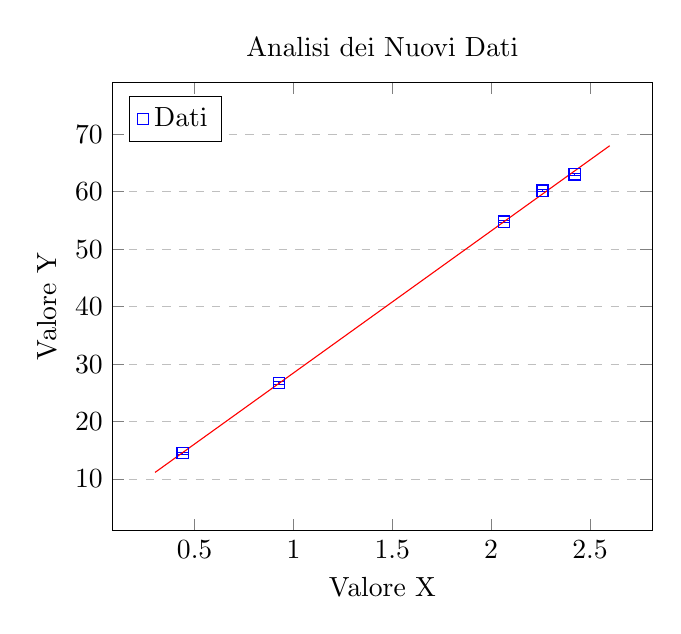
\begin{tikzpicture}
		\begin{axis}[
			title={Analisi dei Nuovi Dati},
			xlabel={Valore X},
			ylabel={Valore Y},
			xmin=0.4, xmax=2.5,
			ymin=10, ymax=70,
			xtick={0,0.5,1,1.5,2,2.5},
			ytick={0,10,20,30,40,50,60,70},
			legend pos=north west,
			ymajorgrids=true,
			grid style=dashed,
			enlargelimits=0.15,
			]
			
			\addplot[
			only marks,
			color=blue,
			mark=square,
			error bars/.cd,
			y dir=both, y explicit
			]
			coordinates {
				(2.260011111,60.20) +- (0,0.2)
				(0.9267271111,26.70) +- (0,0.2)
				(0.4391271111,14.50) +- (0,0.2)
				(2.422173444,63.00) +- (0,0.2)
				(2.064011111,54.80) +- (0,0.2)
			};
			\addplot[
			domain=0.3:2.6, 
			samples=100, 
			color=red, 
			] 
			{ 24.7131*x + 3.74511};
			\legend{Dati}
		\end{axis}
	\end{tikzpicture}
\end{figure}
\end{minipage}




\subsubsection{Test del chi quadro}
Visti i risultati ottenuti assumo che la retta trovata di parametri $\mathbf{A}$ e $\mathbf{B}$ si adatti bene all'andamento dei miei dati. Per assicurarmene effettuo un test del $\chi^2$

\paragraph{Ipotesi nulla} La retta $y = A + Bx$ descrive bene l'andamento dei dati osservati sperimentalmente.

\begin{table}[H]
	\centering
	\begin{tabular}{lr} 
		Livello di significatività $\alpha$		&$\quad 0.05$  \\
		Valore di $\chi ^2$             	& $\quad 4.29$       \\
		Numero di gradi di libertà      	& $\quad (6-2) = 4$         \\   
		Valore di $\chi ^2$ critico     	& $\quad 9.49$
	\end{tabular}
\end{table}

\paragraph{Conclusione test} Il valore del $\chi^2$ ottenuto risulta essere minore del valore critico, posso quindi accettare l'ipotesi nulla e affermare che nei livelli di significatività scelti la retta $y = A + Bx$ descrive in modo accettabile l'andamento dei miei dati.

\subsubsection{Test Z}
Infine, appurato che la retta $y = A + Bx$ è una buona rappresentazione dell'andamento dei miei dati, mi interessa capire se l'andamento teorico lo è. Voglio quindi capire se l'equazione 
\[
\sin{\left(\vartheta/2\right)}^2 = 4\frac{T}{T_0} - 4
\]

che ha come parametri teorici
\[
A_\text{teo} = -4 \qquad B_\text{teo} =  \frac{4}{T_0}
\]
si adatta bene ai miei dati. Scelgo quindi un livello di significa $\alpha = 0.05$ con $z_{\text{critico}} = 1.96$ ed eseguo il test.

\paragraph{Ipotesi nulla} I valori $A_{\text{teo}}$, $\mathbf{A}$ e  $B_{\text{teo}}$, $\mathbf{B}$ sono a due a due compatibili.

\begin{table}[H]
	\centering
	\begin{tabular}{@{}rp{3cm}p{2cm}p{2cm}@{}}
		
		&\textbf{Sperimentali} & \textbf{Teorici} & $z_{\text{oss}}$ \\ \cmidrule(r){2-4}
		\textbf{A}	&$-3.68 \pm 0.18 $		& $-4$	& 1.79 \\
		\textbf{B}	&$2.16 \pm  0.10$		& $4/T_0$ 		& 1.78 \\
	\end{tabular}
\end{table}

\paragraph{Conclusione test} Poiché sia per $\mathbf{A}$ sia per $\mathbf{B}$ risulta che $z_{\text{oss}}$ < $z_{\text{critico}}$ posso affermare che entrambi sono compatibili con i rispettivi valori teorici nei livelli di significaticità scelti e che quindi l'equazione teorica della retta è una buona rappresentazione dell'andamento dei miei dati.



%%%%%%%%%%%%%%%%%%%%%%%%%%%%%%%%%%%%%%%%%%%%%%%%%%%%%%%%%
%%				DIPENDENZA MASSA     MMMM
%%%%%%%%%%%%%%%%%%%%%%%%%%%%%%%%%%%%%%%%%%%%%%%%%%%%%%%%%

\newpage
\section{Dipendenza dalla massa}
Come si può osservare dall'equazione del periodo, questo non è teoricamente influenzato dalla massa appesa ad esso. Tuttavia, sperimentalmente, la massa potrebbe portare a delle più o meno lievi variazioni







%%%%%%%%%%%%%%%%%%%%%%%%%%%%%%%%%%%%%%%%%%%%%%%%%%%%%%%%%
%%				    CONCLUSIONI
%%%%%%%%%%%%%%%%%%%%%%%%%%%%%%%%%%%%%%%%%%%%%%%%%%%%%%%%%

\newpage
\section{Conclusioni}



\end{document}
